% This is part of Un soupçon de physique, sans être agressif pour autant
% Copyright (C) 2006-2010
%   Laurent Claessens
% See the file fdl-1.3.txt for copying conditions.

\thispagestyle{empty}
\title{Un soupçon de physique, sans être agressif pour autant}
\author{Laurent \textsc{Claessens}}
\maketitle

Copyright (c) 2006-2010  Laurent Claessens.

Permission is granted to copy, distribute and/or modify this document under the terms of the GNU Free Documentation License, Version 1.3 or any later version published by the Free Software Foundation; with no Invariant Sections, no Front-Cover Texts, and no Back-Cover Texts. A copy of the license is included in the section entitled ``GNU Free Documentation License''.

The \href{http://gitorious.org/echa}{\LaTeX\ source files} is hosted on \href{http://fr.wikipedia.org/wiki/Git}{gitorious}. A \href{http://student.ulb.ac.be/~lclaesse/echa.pdf}{pdf} version is also available on \href{http://student.ulb.ac.be/~lclaesse/}{my website}.

\vspace{0.5cm}
The pictures on the cover page may not be under FDL. I found them on Linux related websites, so I hope that they are rather free.

\newpage
\LARGE
\thispagestyle{empty}
\vbox\bgroup
\begin{center}
Composé avec des logiciels libres :\\
GNU/Linux

\makebox[\textwidth][s]{%
 \includegraphics[width=5cm]{meditating_gnu.epsi} \includegraphics[width=5cm]{tux.epsi}  
}\par

\bigskip

Grâce à la prodigieuse distibution (K)Ubuntu\\

\bigskip

%\includegraphics[scale=0.25]{dapper_drake_original.eps}
%\includegraphics[width=6cm]{drake.eps}
%\includegraphics[width=6cm]{EdgyEft2.eps}
%\includegraphics[width=10cm]{fawn.eps}

\makebox[\textwidth][s]{%
\includegraphics[height=8cm]{konqi_kubudoc_hires.eps}  
%
\includegraphics[height=8cm]{Jackalope.eps}  
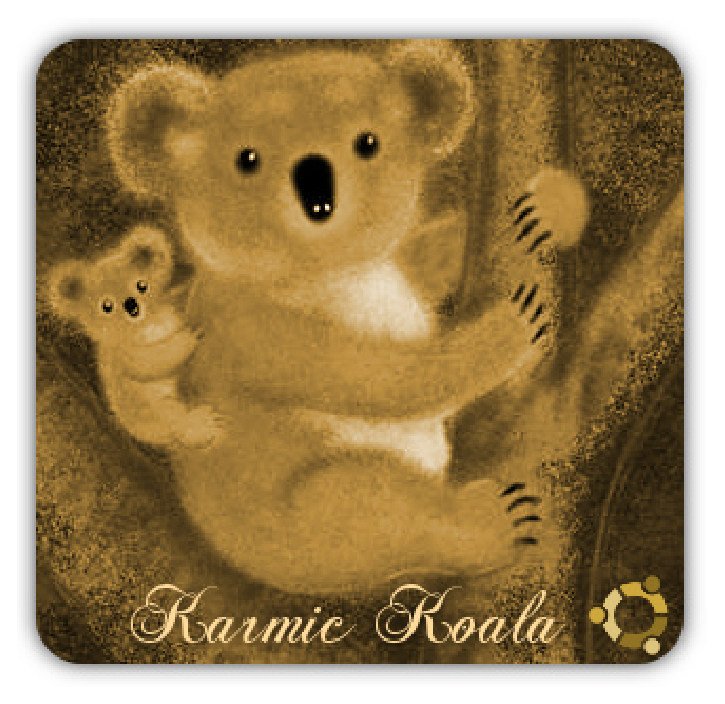
\includegraphics[height=8cm]{koala.eps}  
}\par

\bigskip
 
Et bien entendu\ldots

\bigskip

\includegraphics[width=10cm]{logo.epsi}

\end{center}

\normalsize

\vfill
\noindent
Autre logiciels utilisés : \href{http://fr.wikipedia.org/wiki/PSTricks}{pstricks} pour les figures, avec l'aide de \href{http://fr.wikipedia.org/wiki/Python_(langage)}{python} et \href{http://fr.wikipedia.org/wiki/SAGE_(logiciel_de_calcul_formel)}{Sage} pour la génération de certains bouts de code trop compliqués à programmer en \LaTeX.

\egroup

\normalsize


